\documentclass[11pt]{article}

\usepackage{tikz}

\usetikzlibrary{arrows.meta}

\begin{document}
Hello world? One


\begin{tikzpicture}
\tikz{\draw (0,0) rectangle (2ex, 1em)}
\tikz[very thick] \draw (0,0) rectangle (2ex, 1em); \\
\tikz \draw (0pt, 3pt) -- (20pt, 3pt);
\end{tikzpicture}

\begin{tikzpicture}
\tikz \draw (0pt, 3pt) -- (20pt, 3pt);
\end{tikzpicture}

\begin{tikzpicture}
\tikz \draw[>-] (0pt, 3pt) -- (20pt, 3pt);
\end{tikzpicture}

\begin{tikzpicture}
\tikz \draw[->] (0pt, 3pt) -- (20pt, 3pt);
\end{tikzpicture}

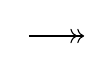
\begin{tikzpicture}
\tikz \draw[->>] (0pt, 3pt) -- (20pt, 3pt);
\end{tikzpicture}

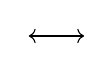
\begin{tikzpicture}
\tikz \draw[<->] (0pt, 3pt) -- (20pt, 3pt);
\end{tikzpicture}

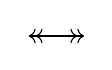
\begin{tikzpicture}
\tikz \draw[<<->>] (0pt, 3pt) -- (20pt, 3pt);
\end{tikzpicture}

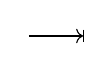
\begin{tikzpicture}
\tikz \draw[->|] (0pt, 3pt) -- (20pt, 3pt);
\end{tikzpicture}

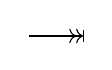
\begin{tikzpicture}
\tikz \draw[->>|] (0pt, 3pt) -- (20pt, 3pt);
\end{tikzpicture}

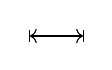
\begin{tikzpicture}
\tikz \draw[|<->|] (0pt, 3pt) -- (20pt, 3pt);
\end{tikzpicture}

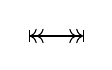
\begin{tikzpicture}
\tikz \draw[|<<->>|] (0pt, 3pt) -- (20pt, 3pt);
\end{tikzpicture}

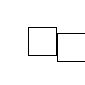
\begin{tikzpicture}
\tikz \draw (0,0) rectangle (1em, 1em);
\tikz[baseline=2pt] \draw (0, 0) rectangle (1em, 1em);
\end{tikzpicture}

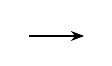
\begin{tikzpicture}
\tikz \draw[-Stealth] (0pt, 3pt) -- (20pt, 3pt);
\end{tikzpicture}

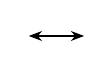
\begin{tikzpicture}
\tikz \draw[Stealth-Stealth] (0pt, 3pt) -- (20pt, 3pt);
\end{tikzpicture}

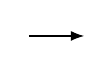
\begin{tikzpicture}
\tikz \draw[-Latex] (0pt, 3pt) -- (20pt, 3pt);
\end{tikzpicture}

\begin{tikzpicture}
\tikz \draw[-{Classical TikZ Rightarrow}] (0pt, 3pt) -- (20pt, 3pt);
\end{tikzpicture}

\tikz{\draw[-{Stealth[length=3mm]}](0,0)--(1.2,0);
\draw[|<->|](0.8,.4) -- node[above=1mm]{3mm}(1.2,.4);}

\tikz{\draw[-{Latex[length=3mm]}](0,0)--(1.5,0);
\draw[|<->|](0.8,.4) -- node[above=1mm]{3mm}(1.2,.4);}

\tikz{\draw[-{Classical TikZ Rightarrow [length=3mm]}](0,0)--(1.2,0);
\draw[|<->|](0.8,0.6) -- node[above=1mm]{3mm}(1.2,.6);}

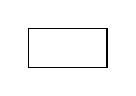
\begin{tikzpicture}
\draw rectangle (1,0.5);
\end{tikzpicture}

\begin{tikzpicture}[x=2, y=1, z=2]
\draw rectangle (2,3);
\end{tikzpicture}

\begin{tikzpicture}[x={(2mm,0)}, y={(0,1mm)}]
\draw rectangle (2,3);
\end{tikzpicture}

\tikz{\draw[line width=5pt] (0,0) -- (1cm, 1.5ex);}
\tikz{\draw[ultra thin] (0,0) -- (1cm,1.5ex);}
\tikz{\draw[very thin] (0,0) -- (1cm, 1.5ex);}
\tikz{\draw[thin] (0,0) -- (1cm,1.5ex);}
\tikz{\draw[semithick] (0,0) -- (1cm, 1.5ex);}

\tikz{\draw[thick] (0,0) -- (1cm, 1.5ex);}
\tikz{\draw[very thick] (0,0) -- (1cm, 1.5ex);}
\tikz{\draw[ultra thick] (0,0) -- (1cm, 1.5ex);}
\tikz{\draw[dash pattern=on 20pt off 3pt on 4pt off 4pt] (0pt, 0pt) -- (50pt, 8pt);}
\tikz{\draw[dash pattern=on 20pt off 8pt, dash phase=0pt](0pt, 0pt) -- (50pt, 8pt);}

\tikz{\draw[dash pattern=on 20pt off 8pt, dash phase=10pt](0pt, 0pt) -- (50pt, 8pt);}
\tikz{\draw[solid](0pt, 0pt) -- (50pt, 8pt);}
\tikz{\draw[dotted](0pt, 0pt) -- (50pt, 8pt);}
\tikz{\draw[densely dotted](0pt, 0pt) -- (50pt, 8pt);}
\tikz{\draw[loosely dotted](0pt, 0pt) -- (50pt, 8pt);}

\begin{tikzpicture}[x=1cm, y=1cm]
\draw[thick, ->] (0,0) -- (5,0); % x 축
\draw[very thick, ->] (2.5, -2.5) -- (2.5, 2.5); % y 축
\draw[color=red](2.5, 0) circle (1.5);
\end{tikzpicture}













\end{document}